\lab{Breadth-First Search}{Breadth-First Search}

\objective{Graph theory has many practical applications. A graph may represent a complex system or network, and analyzing the graph often reveals critical information about the network. In this lab we learn to store graphs as adjacency dictionaries, implement a breadth-first search to identify the shortest path between two nodes, then use the NetworkX package to solve the so-called ``Kevin Bacon problem.''}

\section*{Graphs in Python} % =================================================

Computers can represent mathematical graphs using various kinds of data structures.
In previous labs, we stored graphs as trees and linked lists.
For non-tree graphs, perhaps the most common data structure is an adjacency matrix, where each row of the matrix corresponds to a node in the graph and the entries of the row indicate which other nodes the current node is connected to.
For more on adjacency matrices, see chapter 2 of the Volume II text.

Another common graph data structure is an \emph{adjacency dictionary}, a Python dictionary with a key for each node in the graph.
The dictionary values are lists containing the nodes that are connected to the key.
For example, the following is an adjacency dictionary for the graph in Figure \ref{fig:simple_graph}:

\begin{lstlisting}
# Python dictionaries are used to store adjacency dictionaries.
>>> adjacency_dictionary = {'A':['B', 'C', 'D', 'E'], 'B':['A', 'C'],
'C':['B', 'A', 'D'], 'D':['A', 'C'], 'E':['A']}

# The nodes are stored as the dictionary keys.
>>> print(adjacency_dictionary.keys())
['A', 'C', 'B', 'E', 'D']

# The values are the nodes that the key is connected to.
>>> print(adjacency_dictionary['A'])
>>> ['B', 'C', 'D', 'E']            # A is connected to B, C, D, and E.
\end{lstlisting}

\begin{figure}
\centering
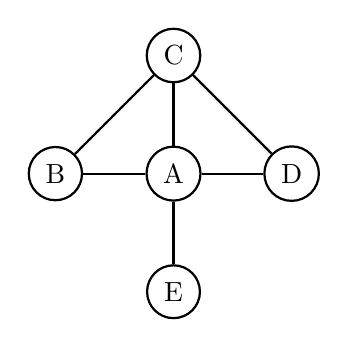
\begin{tikzpicture}[auto,node distance=1.5cm,
 thick,main node/.style={circle,draw}]

  \node[main node] (1) {A};
  \node[main node] (2) [left of=1] {B};
  \node[main node] (3) [above of=1] {C};
  \node[main node] (4) [right of=1] {D};
  \node[main node] (5) [below of=1] {E};

  \path[every node/.style={font=\sffamily\small}]
     (1) edge node [] {} (4)
     	  edge node [] {} (3)
     	  edge node [] {} (5)
     (2) edge node [] {} (1)
     	  edge node []{}(3)
     (3) edge node []{}(4);
\end{tikzpicture}
\caption{A simple graph with five vertices.}
\label{fig:simple_graph}
\end{figure}

% Problem 1: __str__ for Graph class (warmup with dictionaries)
\begin{problem}
Implement the \li{__str__()} method in the provided \li{Graph} class.
Print each node in the graph, followed by a list of the neighboring nodes separated by semicolons.
\\(Hint: consider using the \li{join()} method for strings.)

\begin{lstlisting}
>>> my_dictionary = {'A':['C', 'B'], 'C':['A'], 'B':['A']}
>>> graph = Graph(my_dictionary)
>>> print(graph)
A: C; B
C: A
B: A
\end{lstlisting}
\end{problem}

\section*{Breadth-First Search}

Many graph theory problems are solved by finding the shortest path between two nodes in the graph.
To find the shortest path, we need a way to strategically search the graph.
Two of the most common searches are depth-first search (DFS) and breadth-first search (BFS).
In this lab, we focus on BFS.

A BFS traverses a graph as follows: begin at a starting node.
If the starting node is not the target node, explore each of the starting node's neighbors.
If none of the neighbors are the target, explore the neighbors of the starting node's neighbors.
If none of those neighbors are the target, explore each of their neighbors.
Continue the process until the target is found.

As an example, we will do a programmatic BFS on the graph in Figure \ref{fig:simple_graph} one step at a time.
Suppose that we start at node $C$ and we are searching for node $E$.

\begin{lstlisting}
# Start at node C
>>> start = 'C'
>>> current = start

# The current node is not the target, so check its neighbors
>>> adjacency_dictionary[current]
['B', 'A', 'D']

# None of these are E, so go to the first neighbor, B
>>> current = adjacency_dictionary[start][0]
>>> adjacency_dictionary[current]
['A', 'C']

# None of these are E either, so move to the next neighbor
# of the starting node, which is A
>>> current = adjacency_dictionary[start][1]
>>> adjacency_dictionary[current]
['B', 'C', 'D', 'E']

# The last entry of this list is our target node, and the search terminates.
\end{lstlisting}

You may have noticed that some problems in the previous approach that would arise in a more complicated graph.
For example, what prevents us from entering a cycle?
How can we algorithmically determine which nodes to visit as we explore deeper into the graph?

\subsection*{Implementing Breadth-First Search}

We solve these problems using a queue.
Recall that a \emph{queue} is a type of limited-access list.
Data is inserted to the back of the queue, but removed from the front.
Refer to the end of the Data Structures I lab for more details.

A queue is helpful in a BFS to keep track of the order in which we will visit the nodes.
At each level of the search, we add the neighbors of the current node to the queue.
The \li{collections} module in the Python standard library has a \li{deque} object that we will use as our queue.

\begin{lstlisting}
# Import the deque object and start at node C
>>> from collections import deque
>>> current = 'C'

# The current node is not the target, so add its neighbors to the queue.
>>> visit_queue = deque()
>>> for neighbor in adjacency_dictionary[current]:
...     visit_queue.append(neighbor)
...
>>> print(visit_queue)
deque(['B', 'A', 'D'])

# Move to the next node by removing from the front of the queue.
>>> current = visit_queue.popleft()
>>> print(current)
B
>>> print(visit_queue)
deque(['A', 'D'])

# This isn't the node we're looking for, but we may want to explore its
# neighbors later. They should be explored after the other neighbors
# of the first node, so add them to the end of the queue.
>>> for neighbor in adjacency_dictionary[current]:
...     visit_queue.append(neighbor)
...
>>> print(visit_queue)
deque(['A', 'D', 'A', 'C'])
\end{lstlisting}

We have arrived at a new problem.
The nodes $A$ and $C$ were added to the queue to be visited, even though $C$ has already been visited and $A$ is next in line.

We can prevent these nodes from being added to the queue again by creating a set of nodes to contain all nodes that have already been visited, or that are marked to be visited.
Checking set membership is very fast, so this additional data structure has minimal impact on the program's speed (and is faster than checking the deque).

In addition, we keep a list of the nodes that have actually been visited to track the order of the search.
By checking the set at each step of the algorithm, the previous problems are avoided.

\begin{lstlisting}
>>> current = 'C'
>>> marked = set()
>>> visited = list()
>>> visit_queue = deque()

# Visit the start node C.
>>> visited.append(current)
>>> marked.add(current)

# Add the neighbors of C to the queue.
>>> for neighbor in adjacency_dictionary[current]:
...     visit_queue.append(neighbor)
...     # Since each neighbor will be visited, add them to marked as well.
...     marked.add(neighbor)
...
# Move to the next node by removing from the front of the queue.
>>> current = visit_queue.popleft()
>>> print(current)
B
>>> print(visit_queue)
['A', 'D']

# Visit B. Since it isn't the target, add B's neighbors to the queue.
>>> visited.append(current)
>>> for neighbor in adjacency_dictionary[current]:
...     visit_queue.append(neighbor)
...     marked.add(neighbor)
...

# Since C is visited and A is in marked, the queue is unchanged.
>>> print(visit_queue)
deque(['A', 'D'])
\end{lstlisting}

% Problem 2: general BFS
\begin{problem}
Implement the \li{traverse()} method in the \li{Graph} class using a BFS.
Start from a specified node and proceed until all nodes in the graph have been visited.
Return the list of visited nodes.
If the starting node is not in the adjacency dictionary, raise a \li{ValueError}.
\end{problem}

\section*{Shortest Path} % ====================================================

In a BFS, as few neighborhoods are explored as possible before finding the target.
Therefore, the path taken to get to the target must be the shortest path.

Examine again the graph in Figure \ref{fig:simple_graph}.
The shortest path from $C$ to $E$ is start at $C$, go to $A$, and end at $E$.
During a BFS, $A$ is visited because it is one of $C$'s neighbors, and $E$ is visited because it is one of $A$'s neighbors.
If we knew programmatically that $A$ was the node that visited $E$, and that $C$ was the node that visited $A$, we could retrace our steps to reconstruct the search path.

To implement this idea, initialize a new dictionary before starting the BFS.
When a node is added to the visit queue, add a key-value pair to the dictionary where the key is the node that is visited and the value is the node that is visiting it.
When the target node is found, step back through the dictionary until arriving at the starting node, recording each step.

\begin{problem}
Implement the \li{shortest_path()} method in the \li{Graph} class using a BFS.
Begin at a specified starting node and proceed until a specified target is found.
Return a list containing the node values in the shortest path from the start to the target (including the endpoints).
If either of the inputs are not in the adjacency graph, raise a \li{ValueError}.
\end{problem}

\section*{Network X}

NetworkX is a Python package for creating, manipulating, and exploring large graphs.
It contains a graph object constructor as well as methods for adding nodes and edges to the graph.
It also has methods for recovering information about the graph and its structure.

A node can be an int, a string, or a Python object, and an edge can be weighted or unweighted.
There are several ways to add nodes and edges to the graph, some of which are listed below.

\begin{table}[H]
\centering
\begin{tabular}{r|l}
    Function & Description\\
    \hline
    \li{add_node()} & Add a single node to the graph.\\
    \li{add_nodes_from()} & Add a list of nodes to the graph.\\
    \li{add_edge()} & Add an edge between two nodes.\\
    \li{add_edges_from()} & Add a list of edges to the graph.
\end{tabular}
\end{table}

\begin{lstlisting}
# Create a new graph object using networkX
>>> import networkx as nx
>>> nx_graph = nx.Graph()

>>> nx_graph.add_node('A')
>>> nx_graph.add_node('B')
>>> nx_graph.add_edge('A', 'B')
>>> nx_graph.add_edge('A', 'C') # Node 'C' is added to the graph
>>> nx_graph.add_edges_from([('A', 'D'), ('A', 'E'), ('B', 'C')])

# Graph edges can also have assigned weights.
>>> nx_graph.add_edge('C', 'D', weight=0.5)

# Access the nodes and edges.
>>> print(nx_graph.nodes())
['A', 'C', 'B', 'E', 'D']

>>> print(nx_graph.edges())
[('A', 'C'), ('A', 'B'), ('A', 'E'), ('A', 'D'), ('C', 'B'), ('C', 'D')]

>>> print(nx_graph.get_edge_data('C', 'D'))
{'weight': 0.5}

# Small graphs can be visualized with nx.draw().
>>> from matplotlib import pyplot as plt
>>> nx.draw(nx_graph)
>>> plt.show()
\end{lstlisting}

% Problem 4: Intro to NetworkX
\begin{problem}
Write a function that accepts an adjacency dictionary.
Create a \li{networkx} object, load it with the graph information from the dictionary, and return it.
\end{problem}

\section*{The Kevin Bacon Problem}

\href{http://oracleofbacon.org/help.php}{\emph{The 6 Degrees of Kevin Bacon}} is a well-known parlor game.
The game is played by naming an actor, then trying to find a chain of actors that have worked with each other leading to Kevin Bacon.
For example, Samuel L. Jackson was in the film \emph{Captain America: The First Avenger} with Peter Stark, who was in \emph{X-Men: First Class} with Kevin Bacon.
Thus Samuel L. Jackson has a \emph{Bacon number} of $2$.
Any actors who have been in a movie with Kevin Bacon have a Bacon number of $1$.

% Problem 5: BaconSolver constructor and shortest path
\begin{problem}
Write a \li{BaconSolver} class to solve the Kevin Bacon problem.

The file \texttt{movieData.txt} contains data from about 13,000 movies released over the course of several years.
A single movie is listed on each line, followed by a sequence of actors that starred in it.
The movie title and actors' names are separated by a `/' character.
The actors are listed by last name first, followed by their first name.

Implement the constructor of \li{BaconSolver}.
Accept a filename to pull data from and generate a dictionary where each key is a movie title and each value is a list of the actors that appeared in the movie.
Store the collection of values in the dictionary (the actors) as a class attribute, avoiding duplicates.
Convert the dictionary to a NetworkX graph and store it as another class attribute.
Note that in the graph, actors only have movies as neighbors, and movies only have actors as neighbors.
\\(Hint: recall the \li{split()} method for strings.)
\end{problem}

\begin{warn}
Because of the size of the dataset, \textbf{do not} attempt to visualize the graph with \li{nx.draw()}.
The visualization tool in NetworkX is only effective on relatively small graphs.
In fact, graph visualization in general remains a challenging and ongoing area of research.
\end{warn}

\begin{figure}
\centering
\begin{tikzpicture} [mindmap,every node/.style=concept,concept color=green!60!black,grow cyclic,level 1/.append style={level distance=4cm,sibling angle=90},level 2/.append style={level distance=3cm,sibling angle=45}]

\begin{scope}[text=white]
\node [root concept,scale=.8] {`Bacon, Kevin'}[clockwise from=-5]
	child [concept color=black!70, text=white] {node {Movie}
		child [concept color=green!60!black, text=white] {node {Actor}}
		child [concept color=green!60!black, text=white] {node {Actor}} }
	child [concept color=black!70, text=white] {node {Movie}
		child [concept color=green!60!black, text=white] {node {Actor}} }
	child [concept color=black!70, text=white] {node {Movie}} ;
\end{scope}

\end{tikzpicture}
\caption{A small subgraph demonstrating the structure of the bacon graph.}
\label{fig:bacon_graph}
\end{figure}

NetworkX is equipped with a variety of methods to aid in the analysis of graphs.
A selected few are listed below.

\begin{table}[H]
\centering
\begin{tabular}{r|l}
    Function & Description\\
    \hline
    \li{adjacency_matrix()} & Returns the adjacency matrix as a SciPy sparse matrix.\\
    \li{dijkstra_path()} & Returns the shortest path from a source to a target in a weighted graph.\\
    \li{has_path()} & Returns \li{True} if the graph has a path from a source to a target.\\
    \li{prim_mst()} & Returns a minimum spanning tree for a weighted graph.\\
    \li{shortest_path()} & Returns the shortest path from a source to a target.
\end{tabular}
\end{table}

\begin{lstlisting}
# Verify nx_graph has a path from 'C' to 'E'
>>> nx.has_path(nx_graph, 'C', 'E')
<<True>>

# The shortest_path method is implemented with a
# bidirectional BFS (starting from both ends)
>>> nx.shortest_path(nx_graph, 'C', 'E')
['C', 'A', 'E']
\end{lstlisting}

\begin{problem}
Use NetworkX to implement the \li{path_to_bacon()} method.
Accept start and target values (actors' names) and return a list with the shortest path from the start to the target.
Set Kevin Bacon as the default target.
If either of the inputs are not contained in the stored collection of dictionary values (if either input is not an actor's name), raise a \li{ValueError}.

\begin{lstlisting}
>>> movie_graph = BaconSolver("movieData.txt")
>>> movie_graph.path_to_bacon("Jackson, Samuel L.")
['Jackson, Samuel L.', 'Captain America: The First Avenger', 'Stark,
Peter', 'X-Men: First Class', 'Bacon, Kevin']
\end{lstlisting}
\end{problem}

\begin{problem} % Individual and average Bacon numbers
Implement the \li{bacon_number()} method in the \li{BaconSolver} class.
Accept start and target values and return the number of actors in the shortest path from start to target.
Note that this is different than the number of entries in the shortest path list, since movies do not contribute to an actor's Bacon number.

Also implement the \li{average_bacon()} method.
Compute the average Bacon number across all of the actors in the stored collection of actors.
Exclude any actors that are not connected to Kevin Bacon (their theoretical Bacon number would be infinity).
Return the average Bacon number and the number of actors not connected at all to Kevin Bacon.
\end{problem}

As an aside, the prolific \href{https://en.wikipedia.org/wiki/Erd%C5%91s_number}{Paul Erd\H{o}s} is considered the Kevin Bacon \href{https://xkcd.com/599/}{of the mathematical community}.
Someone with an ``Erd\H{o}s number'' of $2$ co-authored a paper with someone who co-authored a paper with Paul Erd\H{o}s.

\newpage

\section*{Additional Material} % ==============================================

\subsection*{Depth-First Search} % --------------------------------------------

% TODO: Revise this section.
% TODO: Need a (good) picture of a DFS, compared to a BFS.

A \emph{depth-first search} (DFS) takes the opposite approach of a breadth-first search.
Instead of checking all neighbors of a single node before moving, on, it checks the first neighbor, then their first neighbor, then their first neighbor, and so on until reaching a leaf node.
Then the algorithm back tracks to the previous node and checks its second neighbor.
A DFS is sometimes more useful than a BFS, but a BFS is usually better\footnote{\url{https://xkcd.com/761/}} at finding the shortest path.

Consider adding a keyword argument to the \li{traverse()} method of the \li{Graph} class that specifies whether to use a BFS (the default) or a DFS.
This can be done by changing a single line of the BFS code.

\subsection*{Improvements to the BaconSolver Class} % -------------------------

Consider adding a \li{plot_bacon()} method in the \li{BaconSolver} class that produces a simple histogram displaying the frequency of the Bacon numbers in the data set.
% The output should look something like Figure \ref{fig:bacon_numbers}.

% \begin{figure}[H]
%   \includegraphics[width=\textwidth]{figures/baconDistribution.png}
% \caption{The frequency of the bacon numbers.}
% \label{fig:bacon_numbers}
% \end{figure}
% \end{problem}
